%manuel 6e, chapitre G3
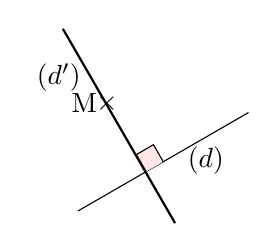
\begin{tikzpicture}[scale=0.5,every node/.style={scale=1},rotate=30]

\draw (0,2) node [left]{M};
\draw (0,2) node {$\times$};
\draw (-2,0)--(3,0) node [near end,below] {$(d)$};
\draw [thick](-0.02,4.2)--(-0.02,-1.5) node[near start,left]{$(d')$};
\draw [fill=pink!40!white](0,0)--(0,0.5)--(0.5,0.5)--(0.5,0);

\end{tikzpicture} 
